\presec
\section{Computing the Optimal k} \postsec
\label{sec:optimalk}

Classically, the optimal number of hash functions is derived through finding the extrema of the asymptotic formula of $f_{bloom}$ given in Eq. \ref{fBloom} as :
\begin{equation}
\label{eq:kopt}
k^*_{bloom}=\frac{m}{n}\ln 2
\end{equation}
However, as we said, the underlying formula for FP probability is not fully correct. In this section, we propose a novel method of deriving the optimal value of $k$, minimizing the FP probability given the value of BF size $m$ and number of inserted elements $n$.


\subsection{Introduction of Information Entropy}
\textbf{Information Entropy}: In information theory, \textit{information entropy} is used to measure the uncertainty of a random variable. In this paper, it refers to the \textit{Shannon entropy} \cite{shannon}, which measures the value of the information contained in a varible.  Entropy is typically measured in bits, nats, or bans \cite{entropy}. For a variable with $s$ events with the probabilities of $p_1$, $p_2$, ..., $p_s$. The information entropy $E$ is defined as:

\begin{equation}
 E=\sum_{i=1}^{s}p_i  log_2 \dfrac{1}{p_i}
\label{equ:entropy}
\end{equation}

\textbf{Property of information entropy:}
For any variable or message, if its information entropy is not at the maximum, it can be compressed without information loss. Suppose a $m$-bit string varible is compressed to $m'$-bit string varible, the entropy becomes $E'$ from $E$. Then we have $mE=m'E'$.
%
% %1) 变量的不确定性越大,熵也就越大
% 1) For a random variable, the larger the uncertainty is, the bigger the information entropy will be.
%
% 2) For any variable or message, there is a maximum value of information entropy.

% 3) When there are some characteristics or regulations in the message, its information entropy is not the maximum.

According to the information entropy formula (Eq. \ref{equ:entropy}), we can obtain the information entropy $E$ of the m-bit varible of a BF:

\begin{equation}
E=-\left(p'\log_2 p' +(1-p')\log_2(1-p')\right)
\label{equ:entropyBF}
\end{equation}
%according to the information entropy formula (Eq. \ref{equ:entropy}), the entropy of BF $h$ is

%\begin{equation}
%h=-\left(p'\log_2 p' +(1-p')\log_2(1-p')\right)
%\end{equation}

\begin{figure}[htbp]
\centering
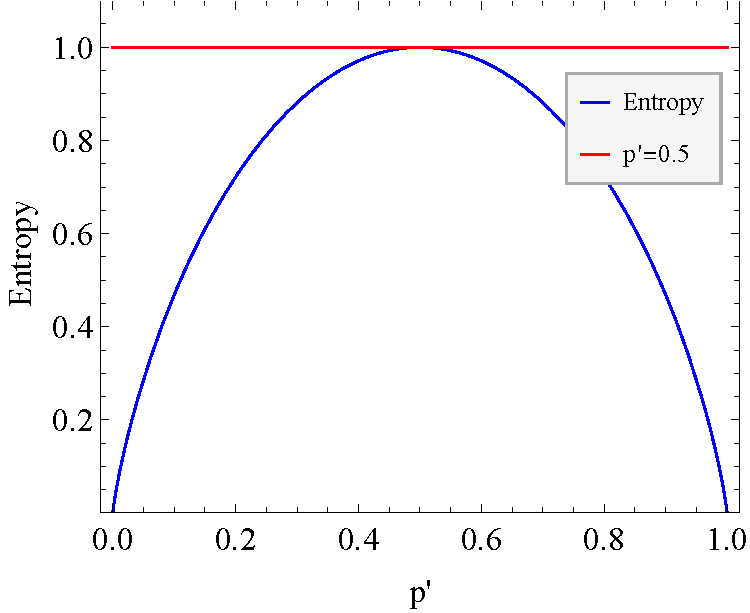
\includegraphics[width=\figwidth]{entropy}
\caption{Information entropy of a BF} \postsec
\label{fig:entropy}
\end{figure}

To be more vivid, we draw the value of $E$ with the increase of $p'$ in Figure \ref{fig:entropy}. Obviously, the maximum value of entropy of an $m$-bit sequence is obtained when the probability that each bit in the BF is 1 (or 0) is 0.5.

%According to Eq. \ref{equ:entropy}, we can obtain the information entropy $h$ of a BF:

%\begin{equation}
%h=-\left(p'\log_2 p' +(1-p')\log_2(1-p')\right)
%\label{equ:entropyBF}
%\end{equation}
%To be more vivid, we draw the Figure of this equation, as shown in Figure \ref{fig:entropy}.
%The function $h$ is a symmetric function and the symmetry axis $p'=0.5$.
%When $p'$ is 0.5, $h$ reaches the maximum value 1. 

%\begin{figure}
%\centering
%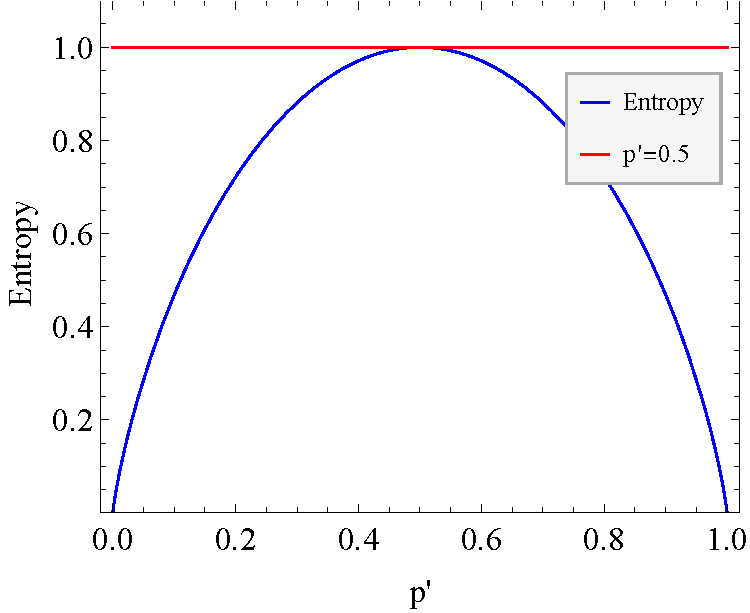
\includegraphics[width=0.8 \linewidth]{entropy}
%\caption{Information entropy of a BF}
%\label{fig:entropy}
%\end{figure}
%Rather than get the exact formula of FP probability, given the value of $m$ and $n$, we deduce the exact formula of the optimal $k$ which Bose's and Christensen's formula cannot get.
%
%According to the theory of information entropy, when there are some characteristics/regulations in the array of BF, the information entropy is not the maximum, and the array can be still compressed without any information loss. Based on this, we have Theorem I.

\subsection{Proposed Theorems about BFs}
\textbf{Lemma I:} Given a BF, suppose $n$ and $k$ keep unchanged, when $m$ becomes larger, the FP probability gets smaller.

\begin{proof}
This lemma is obviously correct. When $n$ and $k$ are fixed, %we expect that 
for larger $m$, the probability of each bit being 1 in the BF becomes smaller, \ie, $p'$ becomes smaller, thus the FP probability gets smaller.
\end{proof}

\textbf{Definition I:} \textit{Bloom filter varible.} The false positive rate of Bloom filters are determined by $m$, $n$, and $k$. For different $n$ elements, the m-bit string varies. Thus when the values of $m$, $n$, $k$ are given, the m-bit string is a random varible. When the $n$ elements are given, the m-bit string is a random varible instance. Therefore, when the values of $m$, $n$, $k$ are given, we call it a Bloom filter varible (BFR). Since it is a random varible, we can compute its information entropy.

\textbf{Definition II:} \textit{Equivalent Bloom filters.} Given two Bloom filters varibles $v_1$ and $v_2$, for any inputting element $y$, $v_1$ reports a vector with $k$ bits, if $v_2$ reports exactly the same $k$ bits, we say $v_1$ and $v_2$ are equivalent.

\textbf{Theorem I:} 
Given a Bloom filter \textit{varible} $v_1$ with parameters $m$, $n$, and $k$, if its information entropy is not at the maximum, there must exist a smaller equivalent Bl\textbf{}oom filter varible $v_2$ with parameters $m'$, $n$ and $k$, where $m'<m$.

\begin{proof}
For $v_1$, the parameters are $m$, $n$, $k$. Suppose its $k$ hash functions are $h_1(\cdot), h_2(\cdot), \ldots, h_k(\cdot)$. 
Since the assumption is that the information entropy of $v_1$ is not at the maximum, according to the property of information entropy, $v_1$ can be compressed \textit{without information loss}. After compression, suppose the new random varible has a length of $m' (m' < m)$\footnote{Note that during the compression, the information value $m*E$ keeps unchanged, while $E's$ maximum value is 1, thus the length of the compressed message has a minimum value.}, we name it $v_2$.

$v_1$ and $v_1$ are two varibles consisting of bits, and we can regard them as two integers varible. We use $In(v_1)$ and  $In(v_2)$ to represent the corresponding integer value of $v_1$ and $v_2$.
Therefore, we use $|In(v_1)|$ represents the length of $v_1$, then we have  $|In(v_1)|=m$, $|In(v_2)|=m'$.
Because we compress $v_1$ and get $v_2$, this can be regarded as a function $g(\cdot)$. In other words, $g(In(v_1))=In(v_2)$. We can also obtain $v_1$ by equation $In(v_1)=g^{-1}(In(v_2))$.

At this stage, we consider the new Bloom filter varible $v_2$, the parameters are $m'$, $n$, and $k$. Note that we use $k$ \texttt{different} hash functions, and the $k$ hash functions are
\begin{equation}
\begin{aligned}
&g^{-1}(In(v_2))\ll h_1(y) \gg (|g^{-1}(In(v_2))|-h_1(y)-1), \\
&g^{-1}(In(v_2))\ll h_2(y) \gg (|g^{-1}(In(v_2))|-h_2(y)-1), \\
& \ldots \\
&g^{-1}(In(v_2))\ll h_k(y) \gg (|g^{-1}(In(v_2))|-h_k(y)-1)
\end{aligned}
\label{equ:g(k)}
\end{equation}
Where $\ll$ means left shift and $\gg$ means right shift.

Given an inputting element $y$, we can compute above $k$ values ONLY using $v_2$ and $h_i(\cdot)$ without $v_1$.
Then we need to prove that for any incoming element $y$, $v_2$ reports the same $k$-bit value.
Let focus on formula \ref{equ:g(k)}, we use equation $v_1=g^{-1}(In(v_2))$ and $m=|g^{-1}(In(v_2))|$, these $k$ hash functions are simplified as

\begin{equation}
\begin{aligned}
&v_1\ll h_1(y) \gg (m-h_1(y)-1), \\
&v_1\ll h_2(y) \gg (m-h_2(y)-1), \\
& \ldots \\
&v_1\ll h_k(y) \gg (m-h_k(y)-1)
\end{aligned}
\label{equ:g(k):simple}
\end{equation}
Here $1\leqslant i\leqslant k$ and $0\leqslant h_i(y)\leqslant m-1$. 
 $v_1\ll h_i(y) \gg (m-h_i(y)-1)$ actually means the value of $h_i(y)$-th bit of $v_1$. 
This is the same as the $k$ hash functions as $v_1$. Therefore, $v_1$ and $v_2$ are equivalent.
\end{proof}

\textbf{Theorem II:} Given a Bloom filter varible, if its information entropy is not at the maximum, the FP probability is definitely not at the minimum.
\begin{proof}
Given a Bloom filter varible $v_1$ with parameters $m$, $n$, $k$. Since the assumption is that the information entropy of $v_1$ is not at the maximum, according to Theorem I, there exists a smaller Bloom filter varible $v_2$ with parameters $m'$, $n$, $k$. Since $v_2$ and $v_1$ are equivalent, their FP probabilities are the same, we name it $f$.
At this stage, we enlarge the size of $v_2$ a little from $m'$ to $m''$, where $m'<m''<m$. According to Lemma I, we know the FP probability of $v_2$ becomes smaller than $f$. This means for $v_1$, there exists a BF varible with smaller size, but with a smaller FP probability. Therefore, the FP probability of $v_1$ is not at the minimum.
\end{proof}


\textbf{Theorem III: contrapositive of Theorem II.} Given a Bloom filter varible, if the FP probability is at the minimum, its information entropy must be at the maximum.
\begin{proof}
This is the contrapositive statement of Theorem II, thus it naturally holds.
\end{proof}

\textbf{Theorem IV: converse of Theorem II.} Given a Bloom filter varible, if the FP probability is not at the minimum, its information entropy must be not at the maximum.
\begin{proof}
Given a Bloom filter varible $v_1$ with parameters $m$, $n$, $k$. Since the assumption is that the FP probability of $v_1$ is not at the maximum, there exists an optimal Bloom filter varible $v_0$ with parameters $m$, $n$, $k'$, where $k'\neq k$. According to Theorem III, the information entropy of $v_0$ is at the maximum. According to Eq. \ref{equ:entropyBF} and Figure \ref{fig:entropy}, the $p'$ of $v_0$ is 0.5, while the $p'$ of $v_1$ is not, because they have different value of $k$. Therefore, the information entropy of BF$_1$ is not at the maximum.
\end{proof}


\textbf{Theorem V: contrapositive of Theorem IV.} Given a Bloom filter varible, if its information entropy is at the maximum, the FP probability is at the minimum. 
%\textbf{To kave: this is what we want, the most important one.}
\begin{proof}
This is the contrapositive proposition of Theorem IV, thus it naturally holds.
\end{proof}



%\textbf{Converse of Theorem III:} Given a Bloom filter, if its information entropy is at the maximum, the FP probability is at the minimum.
%
%\begin{proof}
%This is the converse statement of Theorem III. Because there is only one case the information entropy is at the maximum: $p' =0.5$. Therefore, only when $p'=0.5$, the information entropy is at the maximum, and in this case, the FP probability is at the minimum.
%\end{proof}

%\textbf{Deduction I:} Given a Bloom filter, if $m$ and $n$ are fixed, when $k$ changes, different value of $k$ result in different value of information entropy. Larger information entropy means smaller FP probability.  
%\begin{proof}


%Given a Bloom filter BF$_1$ with parameters $m_1$, $n$, $k_1$ and $v_1$. Suppose its information entropy is $h_1$. If $h_1$ is less than 1 (the maximum value), A can be compressed. After compressed, the memory size becomes $m_2$, and the entropy becomes $h_2$. As we guarantee there is no information loss during the compression, thus $h_1*m_1=h_2*m_2$. Because $m_2<m_1$, thus $h_2<h_1$. 
%
%
%After compressed, the information entropy becomes $h_1$, the memory becomes $m_1$. As we guarantee there is no information loss during the compression, thus $h*m=h_1*m_1$. Because $m_1<m$, thus $h_1>h$. Using the similar method with the proof of theorem I, we can find a new group of $k$ hash functions, and build a new BF, BF$_2$ with parameter $m_1$, $n$, $k$ and A. 


%\end{proof}

%因为压缩后熵变大,
\subsection{Computing the Optimal k}

According to Theorem V, when the information entropy of the Bloom filter varible is at the maximum, the FP probability is at the minimum. Recalling the definition of $p'$ in Eq. \ref{p'form}, one can use this interpretation to find $k^*$, \textit{i.e.}, the optimal number of hash functions. From Figure \ref{fig:entropy}, we know that when $p'$ is 0.5, $E$ reaches the maximum value 1. By setting  the value of $p'$ to 0.5:


% We need to use the\textit{theory of information entropy} to deduce the formula of $k$, thus introduce its basic principle first.

% \textbf{Information Entropy}: In information theory, information entropy is used to measure the uncertainty of a random variable. In this paper, it refers to the \textit{Shannon entropy} \cite{shannon}, which measures the value of the information contained in a message.  Entropy is typically measured in bits, nats, or bans \cite{entropy}. For a variable with $s$ events with the probabilities of $p_1$, $p_2$, ..., $p_s$. The information entropy is:

% \begin{equation}
% p'=\sum_{i=1}^{s}p_i  log_2 \dfrac{1}{p_i}
% \end{equation}

% Here we give some conclusions about information entropy:

% %1) 变量的不确定性越大,熵也就越大
% 1) For a random variable, the larger the uncertainty is, the bigger the information entropy will be.

% 2) For any variable or message, there is a maximum value of information entropy.

% 3) When there are some characteristics or regulations in the message, its information entropy is not the maximum.

% Rather than get the exact formula of FP probability, given the value of $m$ and $n$, we deduce the exact formula of the optimal $k$ which Bose's and Christensen's formula cannot get.

% According to the theory of information entropy, when there are some characteristics/regulations in the array of Bloom Filter, the information entropy is not the maximum, and the array can be still compressed without any information loss. Based on this, we have Theorem I.

% \textbf{Theorem 1: } For a Bloom Filter, if its information entropy is not the maximum, then it is not optimal in size.

% \begin{proof}
% Given a set with $n$ elements, we build a BF with parameters of $m_1$ and $k$, its FP probability is $f_1$. We can compute its entropy. Assuming the entropy is not the maximum, according to the theory of entropy, the BF can be compressed into a smaller one BF2 ($m2 (m2<m1)$ , $k$, $f2$) without any information loss. The FP probability of BF2 is $f_2$, and $f_1=f_2$, because no information is lost during the compression.
% \end{proof}

% In other words, originally we have $m_1$, $k$, when $m_1$ bits are compressed to $m_2$ bits, $n$, $k$ and $f$ are not changed. That is to say, $m_1-m_2$ memory is wasted, thus the value of $k$ is not optimal for the BF with $m$ bits.

% It can be concluded that when there is no characteristic/regulation in the array, its information entropy is the maximum, and the value of $k$ is optimal given $m$ and $n$. Obviously, when the probability that every bit in the BF is 1 is 0.5, it has no characteristic/regulation, its information entropy reaches the maximum, and the value of $k$ is the optimal - $k^*$:
\begin{equation}
p'=\left(1-\frac{1}{m}\right)^{k^* n}=0.5
\label{equ:p=0.5}
\end{equation}
%$$
which is derived previously with the first independence assumption that is not disputed, we obtain:
\begin{equation}
\label{equ:mykform}
k^*=-\dfrac{\ln 2}{n} / \ln\left(1-\dfrac{1}{m}\right)
\end{equation}
This formula is very close to the formula of $k^*$ obtained by Bloom. As we have, as for small values of $x$, the approximation $\ln(1+x)\approx x$, and therefore $-1/\ln(1-\dfrac{1}{m}) \approx m$ yielding the same term as in Eq. \ref{eq:kopt}.


\textbf{Theorem VI:} Given any BF varible, when $m$ and $n$ are fixed, the FP probability $f$ is a function of $k$, we represent it $f(k)$. We claim that $f(k)$ is a \textit{convex function}.

\textit{Note that here a convex function means it has only one minimum value.}
\begin{proof}
Given a Bloom filter varible $v_1$ with parameters $m$, $n$, $k_1$, its entropy is $E_1$.
Given another Bloom filter varible $v_2$ with parameters $m$, $n$, $k_2$, its entropy is $E_2$.

1) For any $k_1<k_2\leqslant k^*$, according to Eq. \ref{p'form}, Eq. \ref{equ:entropyBF} and Figure \ref{fig:entropy}, we known $p'_1<p'_2\leqslant 0.5$.
We compress $v_1$ to $v_3$ with parameters $m_3$, $n$, $k_1$. In order to make $v_3$'s entropy equal to $E_2$, $m_3$ should be $mE_1/E_2$. In this case, the entropy of $v_3$ is equal to that of $v_2$. When the entropy of BF varibles is less than 0.5, same entropy leads to same $p'$. In other words, $p'_3=p'_2$. Because $v_2$ has more hash functions ($k_2>k_1$), thus the FP probability of $v_2$ is smaller than that of $v_3$. While $v_3$ and $v_1$ have the same FP probability, therefore, the FP probability of $v_2$ is smaller than that of $v_1$.
In other words, for any $k (k<k^*)$ increasing, the FP probability of BFs decreases.

2) For any $k*\leqslant k_1<k_2$, according to Eq. \ref{p'form}, Eq. \ref{equ:entropyBF} and Figure \ref{fig:entropy}, we known $p'_1>p'_2\geqslant 0.5$. 
Using the similar derivation, we can derive that the FP probability of $v_2$ is larger than that of $v_1$.

According to the above two cases, we know that given any BF varbile, when $m$ and $n$ are fixed, the FP probability $f$ is a function of $k$, we represent it $f(k)$.  $f(k)$ is a \textit{convex function}.
\end{proof}

%yt: this Theorem is not correct for all cases, I need to think more.
%\textbf{Theorem VII:} Given two BFs with same value of $k$, if their information entropy are the same, their FP probabilities are the same. 
%\begin{proof}
%Given a Bloom filter BF$_1$ with parameters $m_1$, $n_1$, $k_1$, $p'_1$, its entropy is $h$.
%Given another Bloom filter BF$_2$ with parameters $m_2$, $n_2$, $k_2$, $p'_2$, its entropy is $h$.
%Because they have the same entropy $h$, thus $p'_1=p'_2$ or $p'_1+p'_2=1$. In addition, they have same number of hash functions, i.e., $k_1=k_2$, thus $p'_1=p'_2$. According $k_1=k_2$ and $p'_1=p'_2$, the FP probability of BF$_1$ and BF$_2$ are the same.
%\end{proof}
